\begin{tikzpicture}[overlay, remember picture]
    \node[anchor=north west, rotate=0, gray, font=\tiny, text width=\paperwidth] at (current page.south west)  [xshift=0, yshift=1.5cm] {
    [2] A. Bergschneider et al., Experimental Characterization of Two-Particle Entanglement through Position and Momentum Correlations, Nature Physics 15, no. 7 (2019)

    \only<3,4>{
    [3] M. Jafarpour et al., A Useful Strong Lower Bound on Two-Qubit Concurrence, Quantum Information Processing 11, no. 6 (2012)
    }
    };
\end{tikzpicture}

% Jafarpour, Mojtaba, and Abbass Sabour. ‘A Useful Strong Lower Bound on Two-Qubit Concurrence’. Quantum Information Processing 11, no. 6 (December 2012): 1389–1402. https://doi.org/10.1007/s11128-011-0288-0.


% \begin{figure}[h]
%     \centering
%     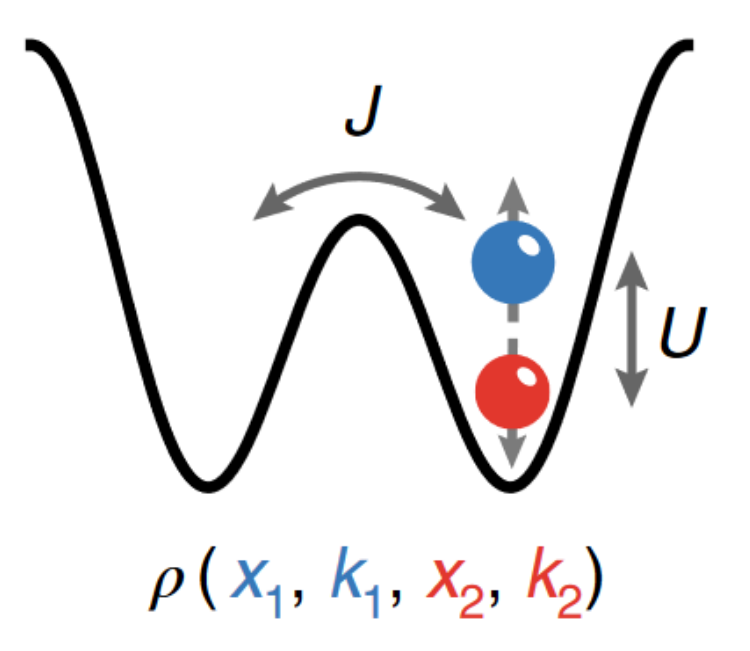
\includegraphics[width=0.5\textwidth]{imgs/Exp1.png}
%     %\caption{}
%     %\label{fig:}
% \end{figure}


% , Andrea, Vincent M. Klinkhamer, Jan Hendrik Becher, Ralf Klemt, Lukas Palm, Gerhard Zürn, Selim Jochim, and Philipp M. Preiss. ‘’. Nature Physics 15, no. 7 (July 2019): 640–44. https://doi.org/10.1038/s41567-019-0508-6.

%  \begin{tikzpicture}[overlay, remember picture]
%         \node[circle, fill=black, inner sep=2pt, label=above:$A$] at (current page.north east) [xshift=-2cm, yshift=-1.5cm] (A) {};
%         \node[circle, fill=black, inner sep=2pt, label=above:$B$] at (current page.north east) [xshift=-1cm, yshift=-1.5cm] (B) {};
%         \draw (A) -- (B);
% \end{tikzpicture}

\only<1>{
Consider dimer system
	\begin{figure}[h]
	    \centering
	    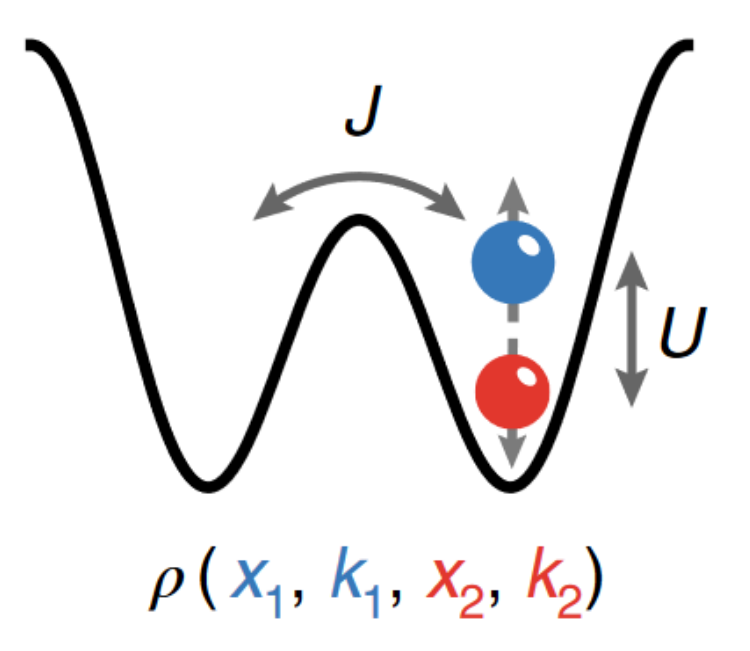
\includegraphics[width=0.3\textwidth]{imgs/Exp1.png}
	    %\caption{}
	    %\label{fig:}
	\end{figure}
With Hamiltonian
}
\only<1,2,3,4>{
\only<2,3,4>{\vspace{-1cm}}
\begin{equation*}
	\hat{H} = - J \sum_\sigma \left(\hat{c}_{\text{L} \sigma} \hat{c}_{\text{R} \sigma} + \text{c.c.}\right) + U \sum_{j=\text{L,R}} \hat{n}_{j \downarrow} \hat{n}_{j \uparrow}
\end{equation*}

% \phantom{42}


}
\only<2,3,4>{
What is available for us to measure?
\begin{minipage}{0.45\textwidth}
\begin{figure}[h]
    \centering
    \only<2,3,4>{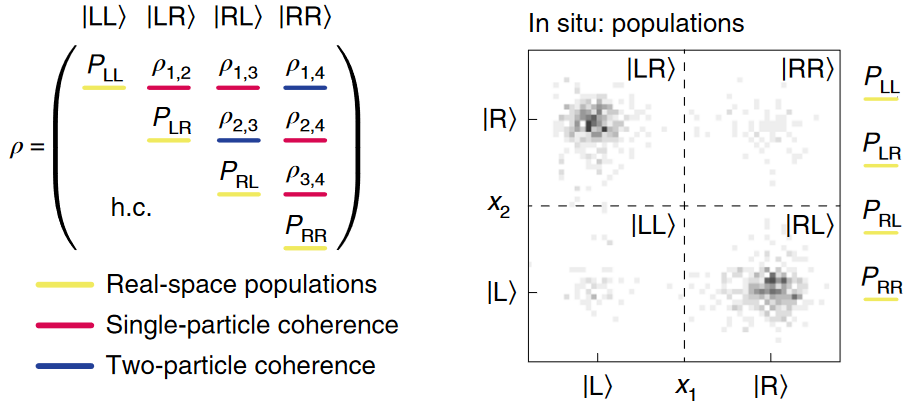
\includegraphics[width=\textwidth]{imgs/Exp4.png}}
    %\caption{}
    %\label{fig:}
\end{figure}
\end{minipage}
\hfill
\begin{minipage}{0.45\textwidth}
\begin{figure}[h]
    \centering
    \only<2,3>{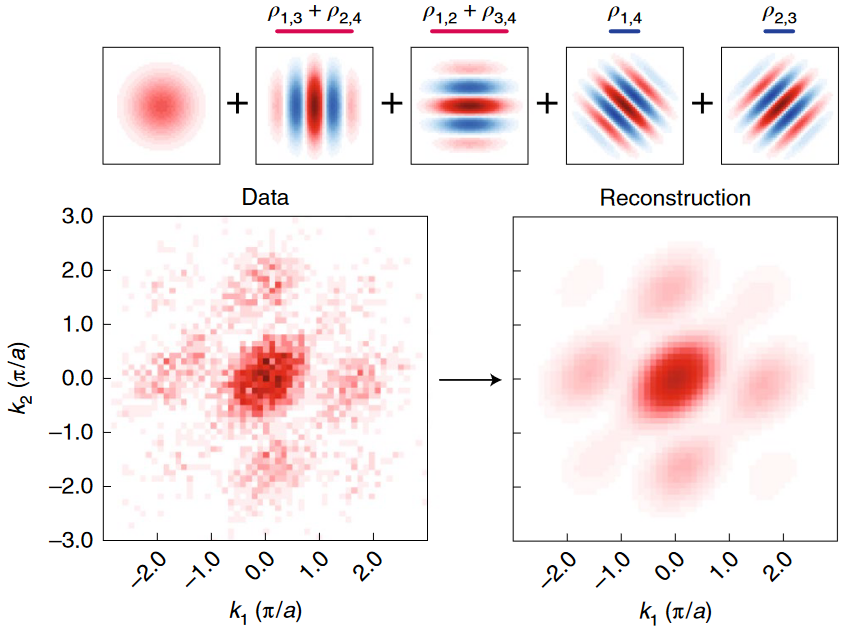
\includegraphics[width=\textwidth]{imgs/Exp2.png}}
    \only<4>{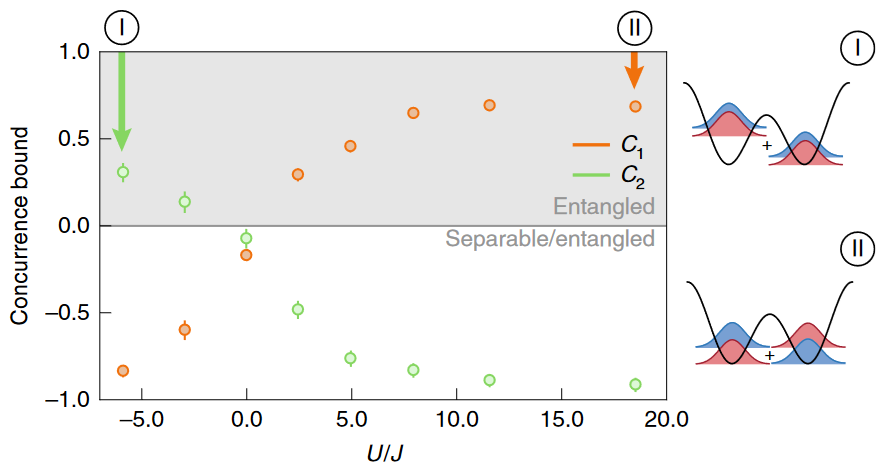
\includegraphics[width=\textwidth]{imgs/Exp3.png}}
    %\caption{}
    %\label{fig:}
\end{figure}
\end{minipage}


\onslide<3,4>{
\only<3>{\vspace{-5mm}}
	Lower bound for concurrence
	\begin{equation*}
		C(\rho) \geq \max\left\{
			0, \
			2(|\rho_{1,4}| - \sqrt{\sub{P}{LR} \sub{P}{RL}}),\
			2(|\rho_{2,3}| - \sqrt{\sub{P}{LL} \sub{P}{RR}})
		\right\}
	\end{equation*}
}

}

